\section{Versuchsaufbau}
\label{sec:Versuchaufbau}
Der Aufbau besteht aus einem geschlossenen Rohrsystem, das mit einer Dopplerphantomflüssigkeit befüllt ist. Das Rohrsystem ist in drei Abschnitte mit unterschiedlichen Rohrinnendurchmessern unterteilt. Um die Flüssigkeit in Bewegung zu setzen ist eine Pumpe angeschlossen, an der seitlich durch ein Regler die Geschwindigkeit in Prozent eingestellt wird. Für die Erzeugung des Ultraschalls wird ein Ultraschall Doppler-Generator mit einer $\SI{2}{\mega\hertz}$ Ultraschallsonde verwendet. Mit dem Programm $\emph{Flowview}$ werden die Daten analysiert und graphisch dargestellt. Alle verwendeten Objekte sind in Abbildung \ref{fig:} dargestellt.

\begin{figure}
  \centering
  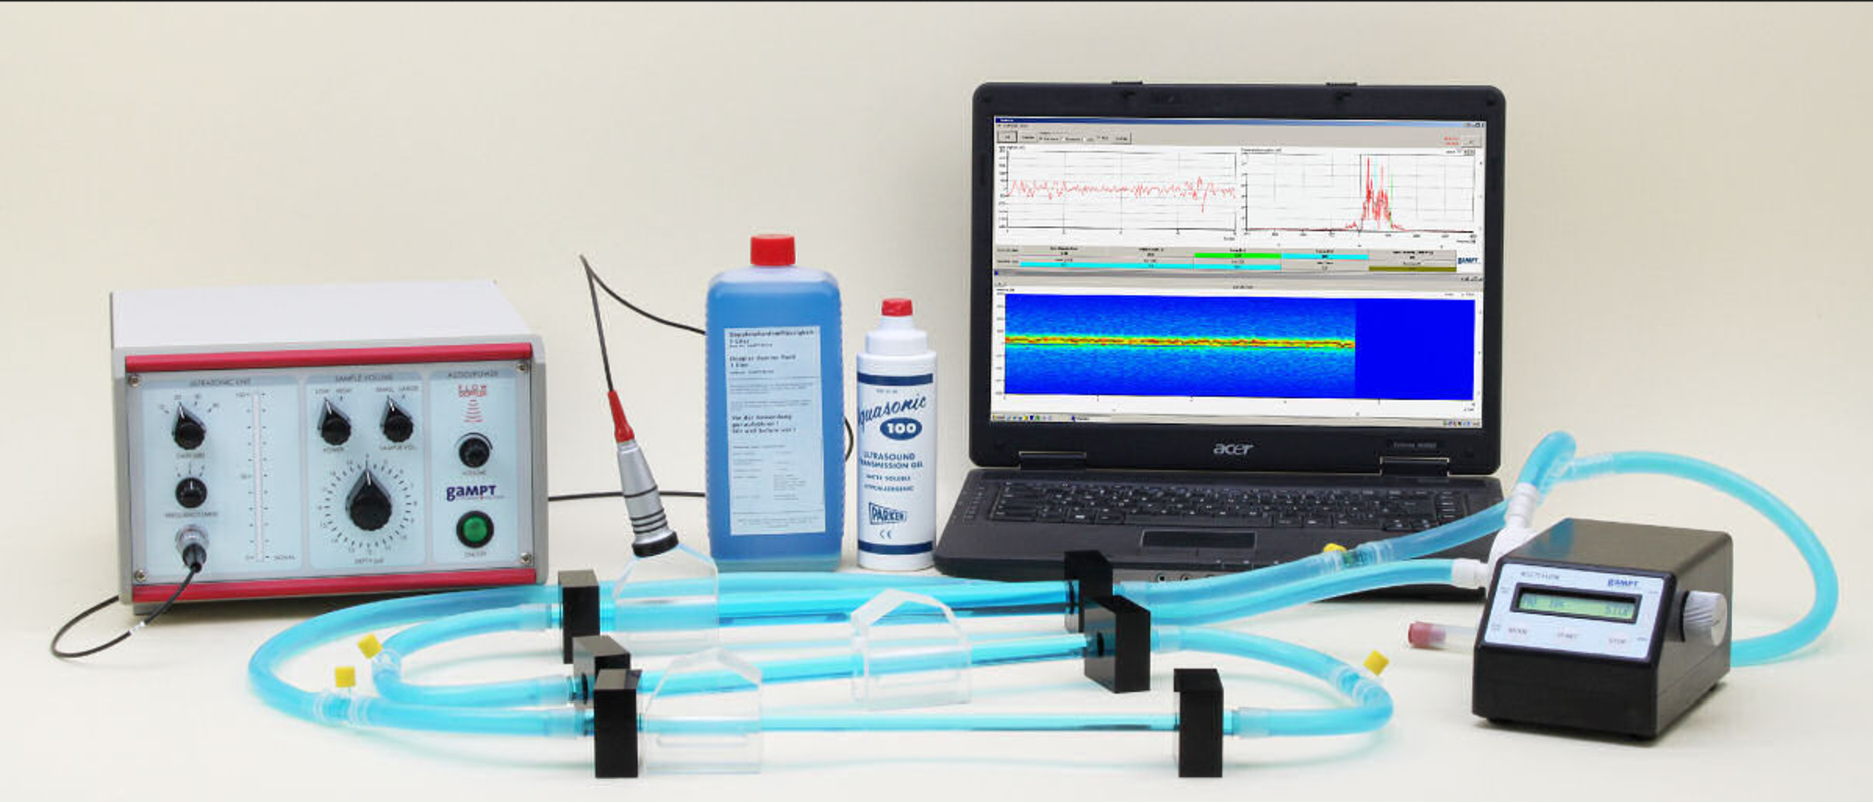
\includegraphics[width=\textwidth]{ressources/Aufbau.pdf}
  \caption{Verwendete Objekte, \cite{skript}.}
  \label{fig:Aufbau}
\end{figure}

Für einen konstanten Winkel $\alpha$ werden Doppler-Prismen mit jeweils drei Einschallwinkeln verwendet, siehe Abbildung $\ref{fig:Prisma}$. Für die jeweiligen Dopplerwinkel gilt
\begin{align}
  \alpha = 90 ^\circ - \arcsin{\left( \sin{(\theta)}\frac{c_\textrm{L}}{c_\textrm{P}}\right)} \;.
  \label{eq:Winkel}
\end{align}

\begin{figure}
  \centering
  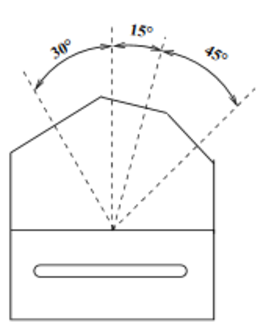
\includegraphics{ressources/Prisma.pdf}
  \caption{Prisma mit drei verschiedenen Winkeln $\Theta$, \cite{skript}.}
  \label{fig:Prisma}
\end{figure}
